\documentclass[12pt]{article}
\usepackage{fullpage}
\usepackage{amsmath}
\usepackage{hyperref}
\usepackage{graphicx}
\usepackage{listings}
\usepackage{float}

\floatstyle{plain}
\newfloat{snippet}{thb}{lop}
\floatname{snippet}{Snippet}


\begin{document}
  \begin{center}
    \textbf{\large Out-of-Order SMIPS} \\
    6.375 Microarchitecture Design Proposal\\
    6 April 2011 \\
    
    \vspace{\baselineskip}
    
    \emph{Team}: David S. Greenberg and Bhaskar Mookerji
  \end{center}

For our 6.375 final project, we are implementing a superscalar processor using Tomasulo's algorithm.

\section{Problem\label{sec:problem}}

\section{High-Level Design}

\begin{figure}[ht!]
    \centering
    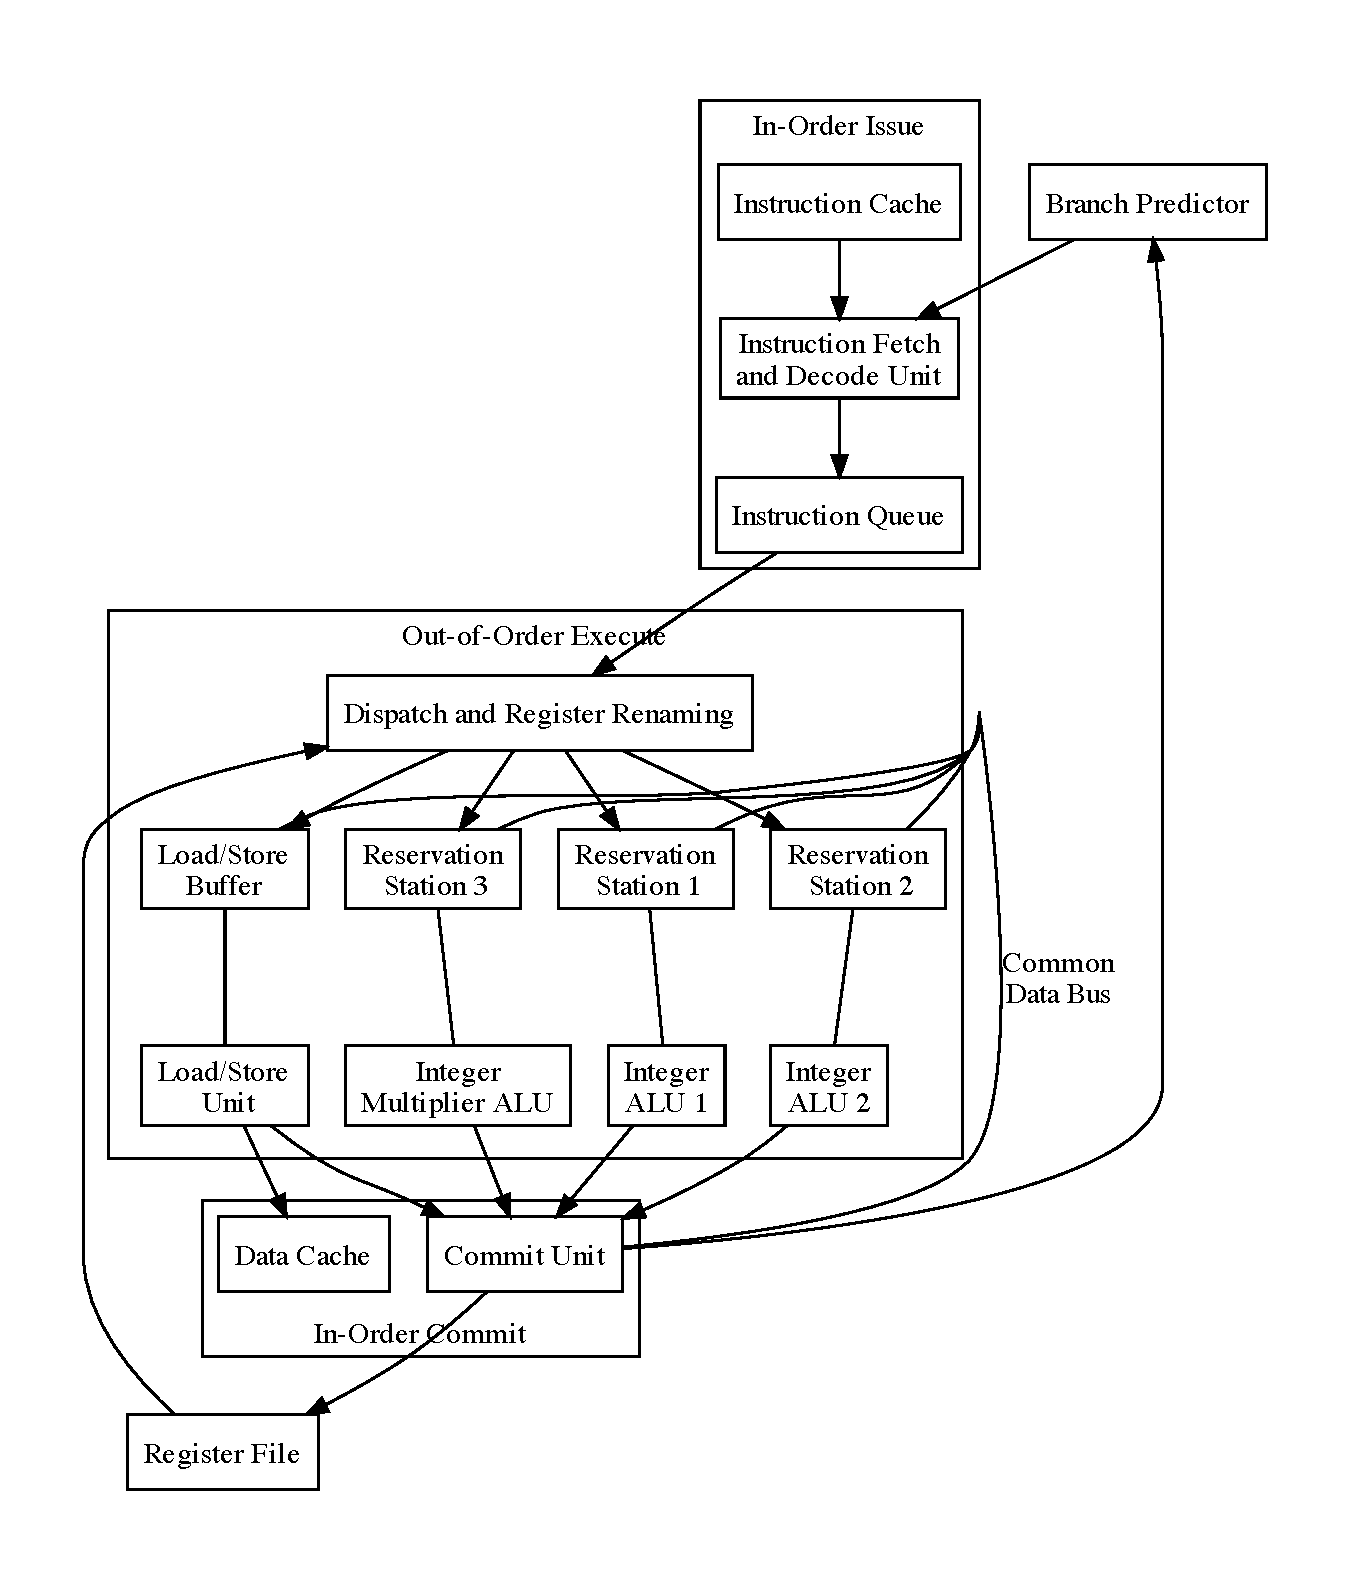
\includegraphics[width=\textwidth]{figures/design.pdf}
    \caption{System architecture using out-of-order execution and pipelined integer arthmetic. \label{fig:design}}
\end{figure}

\begin{figure}[h]
    \centering
    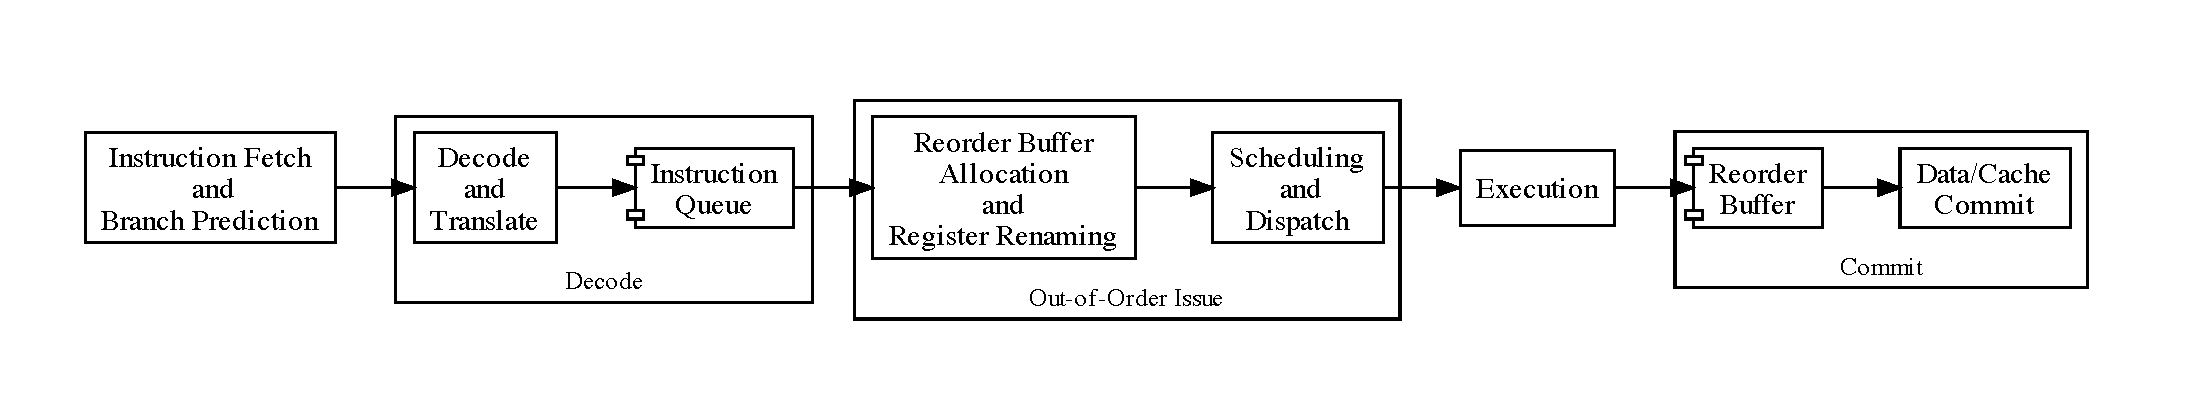
\includegraphics[width=1.1\textwidth]{figures/pipeline.pdf}
    \caption{Instruction pipeline. Pipeline stage is labeled in-box, unless superseded by an overbox. A component box indicates component (such as a FIFO) between stages. Not included in this diagram is the reservation stations and load/store buffer in the execution stage.\label{fig:pipeline}}
\end{figure}



\subsection{FPGA Issues}


 \end{document}
